\section{Theorie}
\label{sec:Theorie}
Licht kann als elektromagnetische Welle interpretiert werden. Durch die Überlagerung
zweier Wellen treten unter bestimmten Bedingungen Interferenzeffekte auf, welche mit
einem Interferometer vermessen werden können. Damit lässt sich die in diesem Versuch
zu untersuchende Größe des Brechungsindex untersuchen.
Eine Lichtwelle kann also wie in Gleichung \ref{eq:Welle} als Funktion von Raum und Zeit
mathematisch ausgedrückt werden. Dabei beschreibt der Vektor $\vec{E_0}$ die Polarisation des Lichtes an.
\begin{equation}
	\vec{E}(\vec{r},t) = \vec{E_0}\cdot \exp i(\omega t - \vec{k}\vec{r})
\label{eq:Welle}
\end{equation}
Der verwendete HeNe-Laser liefert kohärentes, also interferenzfähiges Licht.
Nach dem Superpositionsprinzip addieren sich zwei Wellen in jedem Raumzeitpunkt,
sodass eine überlagerte Welle entsteht. Wenn zwischen den Wellen ein Gangunterschied
$\delta$ existiert treten Interferenzeffekte auf. In einem Michelson-Interferometer wird der
Gangunterschied über die verschieden langen Laufwege der zwei Lichtstrahlen erzeugt, dies ist
beim Sagnac-Interferometer nicht der Fall. Hier wird der Gangunterschied durch das einbringen
einer Probe erzeugt. Die Strahlenarm der durch die Probe geht interferiert mit dem Referenzarm,
der nicht durch die Probe läuft. Der Gangunterschied beider Strahlenarme wird durch die
unterschiedlichen Brechungsindizes herforgerufen.
\subsection{Das Sagnac-Interferometer}
\label{sec:SI}
In Abbildung \ref{fig:Aufbau} ist der Versuchsaufbau schematisch dargestellt. Der
Lichtstrahl aus dem Helium-Neon-Laser wird über zwei Steuerspiegel zunächst auf einen Polarisationsfilter
und dann auf einen Polarizing-Beam-Splitter-Cube (PBSC) gelenkt. Der PBSC besteht aus zwei Prismen, welche
an der Hypotenuse zusammengeklebt sind. Der Lichtstrahl wird ohne nennenswerten Intensitätsverlust
in dem PBSC in zwei Strahlen geteilt,
welche sowohl in der Ausbreitungsrichtung als auch in der Polarisation senkrecht zu einander stehen. Die
so erzeugten Strahlen durchlaufen nun das selbe Rechteck aus Spiegeln, jedoch in unterschiedlicher Richtung.
Sie treffen sich am selben PBSC wie zu Trennung und interferieren dort.\\
Befindet sich eine Probe im Lichtstrahl tritt konstruktive Interferenz auf und die Anzahl der Maxima
kann genutzt werden um den Brechungsindex der Probe zu untersuchen.\\
Die Vermessung der Maxima geschieht durch einen weiteren Durchgang durch einen zweiten PBSC.
Die aufgetrennten Strahlen treffen dann auf Photodioden.
\begin{figure}[H]
  \centering
  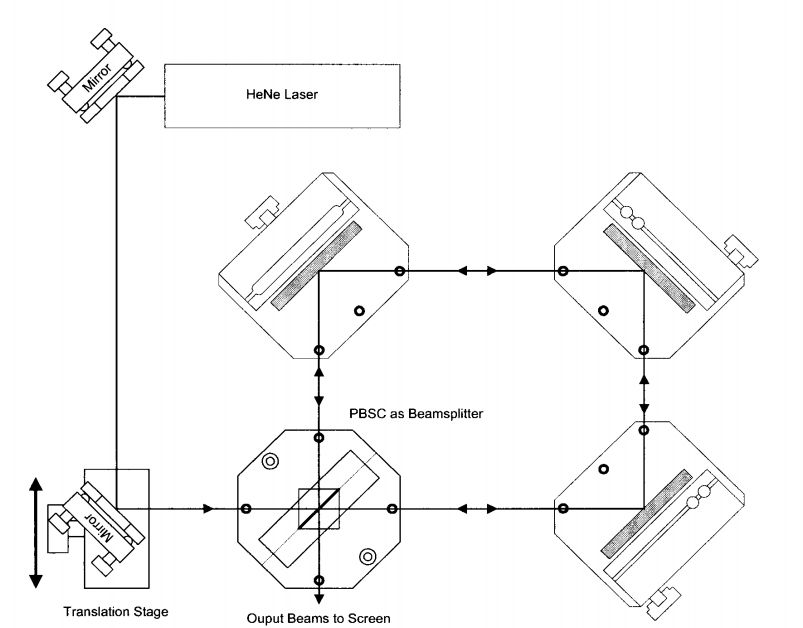
\includegraphics[width=0.6\textwidth]{pics/Aufbau.png}
  \caption{Schematische Darstellung des Sagnac-Interferometers \cite{Anleitung}.}
  \label{fig:Aufbau}
\end{figure}
\subsection{Kontrastbestimmung}
Ein Qualitätsmaß von Interferometern ist der Kontrast K. Dieser wird durch die maximalen
und minimalen Intensitäten mit :
\begin{equation}
	K= \frac{I_{\text{max}}-I_{\text{min}}}{I_{\text{max}}+I_{\text{min}}}
	\label{eq:Kontrast}
\end{equation}
bestimmt. Dabei ist 1 der bestmögliche und 0 der schlechteste Wert. \\
Die Intensität kann mit
\begin{equation}
	I \propto <|E_1 \cos{(\phi)}\cos{(\omega t)} + E_2 \sin{(\phi)}\cos{(\omega t + \delta)} |^2>
\end{equation}
beschreiben werden. Da sie sich  Dabei beschreibt $\phi$ den Polarisationswinkel, $E_0$ die
Amplituden der Wellen und $\delta$ eine Phasenverschiebung.
Für konstruktive bzw. destruktive Interferenz gilt:
\begin{align*}
	\delta_{\text{k}}&=2 n \pi , n \in \mathds{N}_0 \\
	\delta_{\text{d}}&=(2n+1)\pi , n \in \mathds{N} .
\end{align*}
Weiterhin gilt $<\cos(\omega t + \delta)>=1/2$ .
Damit lässt sich die Intensität ausdrücken zu:
\begin{equation}
	I \propto I_{\text{Laser}}\left(1\pm 2\cos{(\phi)}\sin{(\phi)}\right)
\end{equation}
Wobei die Amplituden über die Amplituden des Lasers $I_{\text{Laser}\propto (E_1+E_2)^2}$
ausgedrückt werden.
Daraus kann unter der Verwendung des Additionstheorems $\sin{(2\phi)}=2\cos{(\phi)}\sin{(\phi)}$
die Gleichung \ref{eq:Kontrast} umgeformt werden:
\begin{equation}
	K=\sin{2\phi}
	\label{eq:Kontrast2}
\end{equation}
\subsection{Brechungsindex}
Ist der Kontrast ausreichend hoch, kann über die Abzählung der Interferenz Maxima der
Brechungsindex von Proben bestimmt werden.\\
Die Anzahl der Maxima $M$ lässt sich als Funktion des Phasenversatzes $\Delta \phi$ ausdrücken.
\begin{equation}
	M=\frac{\Delta \phi}{2\pi}
\label{eq:dp}
\end{equation}
Nun sollen zwei Fäll betrachtet werden.
\paragraph{Brechungsindex eines Plättchens}
Wird der Phasenunterschied der beim durchlaufens eines Plättchens mit Brechungsindex $n$ auftritt betrachtet,
wirken dort zwei Effekte. Einmal die Phasenänderung aufgrund des Brechungsindex und einmal die
Phasenverschiebung aufgrund von Brechung. Über die Geometrie des Strahlengangs im Plättchen und durch
Verwendung des Snelius-Relation und der Gleichung \eqref{eq:dp} ergibt sich
\begin{equation}
M \approx \frac{2d}{\lambda_{vac}} \frac{n-1}{n} \theta^2 \; ,
\label{eq:pM}
\end{equation}
dabei bezeichnet $d$ die Dicke des Plättchens, $\lambda_{vac}$ die Vakuumwellenlänge und $\theta$ den
Winkel zwischen Plattennormale und dem eintreffenden Strahl \cite{Anleitung}.
\paragraph{Brechungsindex eines Gases}
Der Phasenunterschied der auftritt wenn das Licht ein Gas durchläuft ist nur auf den Brechungsindex des
Gases zurück zuführen. Also der Übergang von Vakuum $n_{vac}= 1$ zum Gas mit Brechungsindex $n$. Daraus folgt
die Gleichung
\begin{equation}
M = \frac{n-1}{\lambda_{vac}} L \; ,
\label{eq:lM}
\end{equation}
dabei bezeichnet $L$ die Strecke, die das Licht im Gas zurücklegt, also in diesem Aufbau die Länge der Gaszelle
\cite{Anleitung}. Ein anderer Weg den Brechungsindex eines Gases zu bestimmen, ist das Lorentz-Lorenz-Gesetz
\begin{gather}
\frac{n^2 -1}{n^2 +2} = \frac{4\pi}{3} N \alpha_m \\
\text{Nährung:} \quad n \approx \sqrt{1+ \frac{3Ap}{RT}}
\label{eq:NLL}
\end{gather}
dabei bezeichnet $N$ die Teilchenzahl pro Volumen, $\alpha_m$ die molekulare Polarisierbarkeit, $A$ die
molare Polarisierbarkeit, $p$ den Druck, $R$ die allgemeine Gaskonstante und $T$ die Temperatur
\cite{LLG}.
